\section{LEVEL 4 · Samenhang of oorzaak?}

\begin{missie}
Missie: trap niet in de val van ‘het één veroorzaakt het ander’. (LPD 12)
\end{missie}

\begin{doel}
\textbf{DOEL} \quad Na dit level kan je:

☐ \textbf{samenhang} (correlatie) herkennen in een spreidingsdiagram;

☐ in concrete situaties het verschil uitleggen tussen \textbf{samenhang} en \textbf{causaliteit};

☐ een \textbf{verborgen variabele}, een \textbf{omgekeerde oorzaak} of \textbf{toeval} herkennen als verklaring;

☐ \textbf{observationeel} en \textbf{experimenteel} onderzoek onderscheiden en een experiment opzetten met testgroep en controlegroep;

☐ misleidende uitspraken in reclame en nieuws ontmaskeren.
\end{doel}

\subsection*{Theorie 4.1 · Samenhang en causaliteit}

\begin{theorie}
Twee variabelen hebben \textbf{samenhang} (correlatie) als ze samen veranderen.

\begin{itemize}
\item \textbf{Positieve samenhang}: hoe groter de ene, hoe groter de andere (de puntenwolk stijgt).
\item \textbf{Negatieve samenhang}: hoe groter de ene, hoe kleiner de andere (de puntenwolk daalt).
\item \textbf{Geen samenhang}: de punten vormen een wolk zonder richting.
\end{itemize}

\textbf{Causaliteit} betekent dat een verandering in $A$ een verandering in $B$ \emph{veroorzaakt} (oorzaak – gevolg).
\end{theorie}

\begin{center}
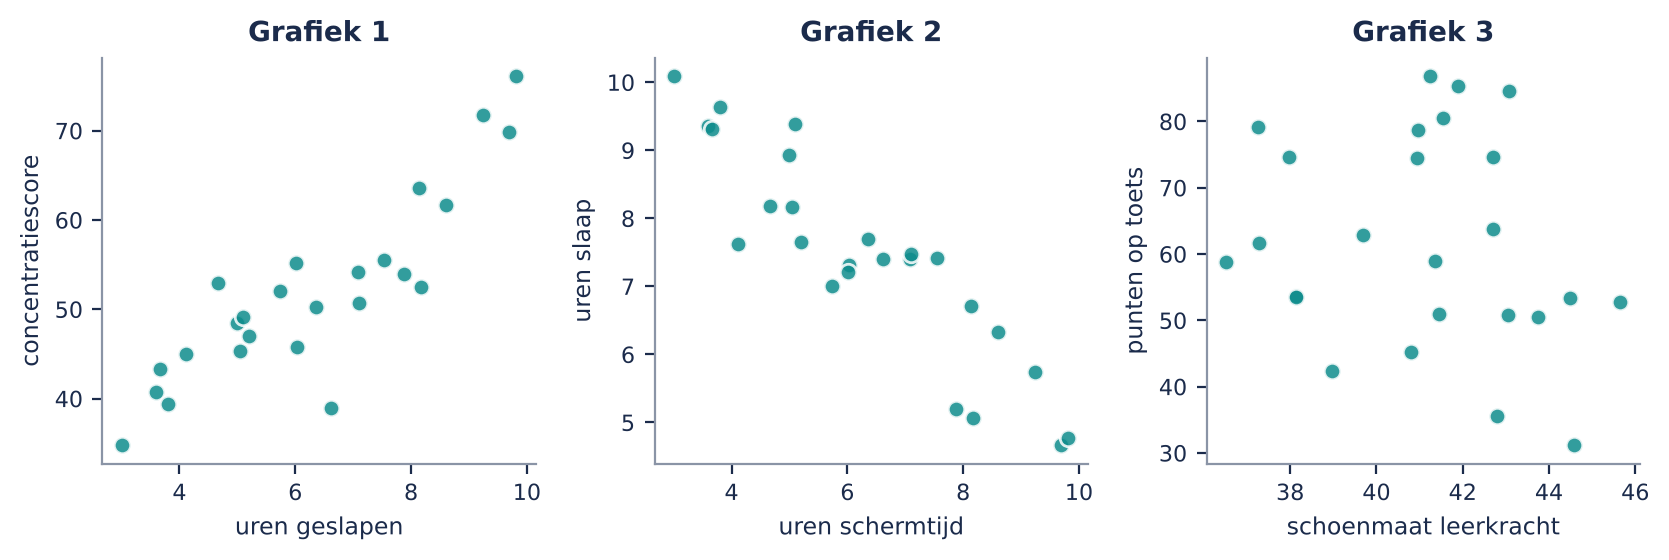
\includegraphics[width=0.95\textwidth]{figuren/l4_spreiding.png}
\end{center}

\begin{letop}
\textbf{LET OP} \quad Samenhang bewijst \textbf{nooit} op zichzelf een oorzaak–gevolg-verband. Vaak wordt samenhang onterecht gelezen als causaliteit.
\end{letop}

\subsection*{Theorie 4.2 · Vier verklaringen voor samenhang}

\begin{theorie}
Als je samenhang vindt tussen $A$ en $B$, zijn er vier mogelijke verklaringen:

\begin{enumerate}
\item \textbf{$A$ veroorzaakt $B$} (echte causaliteit).
\item \textbf{$B$ veroorzaakt $A$} (omgekeerde causaliteit: oorzaak en gevolg zijn omgedraaid).
\item \textbf{Een derde, verborgen variabele $C$ beïnvloedt beide} (\emph{confounding}, ‘verstorende variabele’).
\item \textbf{Toeval}: de samenhang is een toevallige samenloop, zeker bij weinig gegevens of als je naar véél variabelen zoekt.
\end{enumerate}
\end{theorie}

\begin{voorbeeld}
\textbf{Voorbeeld 1: verborgen variabele.} In de zomer worden meer ijsjes verkocht én verdrinken er meer mensen. Ijsjes veroorzaken geen verdrinking: het warme weer zorgt voor allebei.
\end{voorbeeld}

\begin{center}
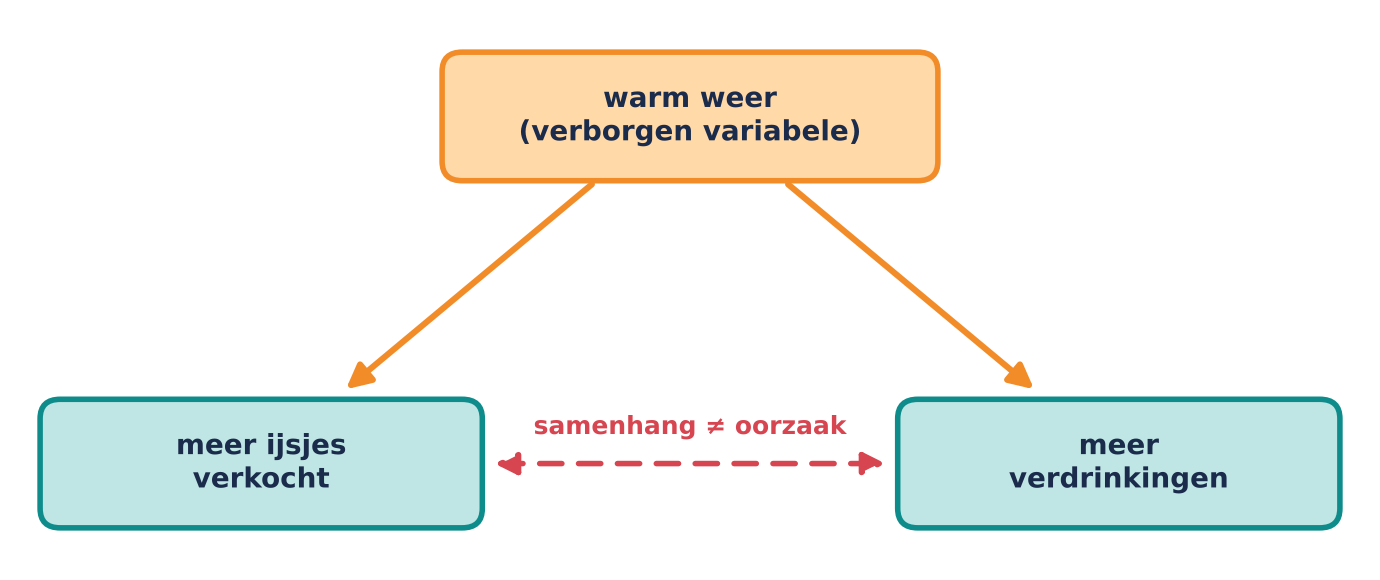
\includegraphics[width=0.75\textwidth]{figuren/l4_verborgen.png}
\end{center}

\begin{voorbeeld}
\textbf{Voorbeeld 2: omgekeerde causaliteit.} Mensen die vaak naar de psycholoog gaan, voelen zich gemiddeld slechter. Niet de psycholoog maakt hen slechter: wie zich slecht voelt, gaat vaker naar de psycholoog.

\textbf{Voorbeeld 3: toeval.} Het aantal geboortes en het aantal ooievaars in een regio hangen samen. Dat komt niet omdat ooievaars baby’s brengen; beide zijn groter in landelijke gebieden (verborgen variabele). Soms is een samenhang louter toeval, zoals twee tendensen over jaren die toevallig gelijk oplopen.
\end{voorbeeld}

\subsection*{Theorie 4.3 · Observationeel en experimenteel onderzoek}

\begin{theorie}
\breedtes{18/41/41}
\begin{tabular}{lll}
\hline
 & observationeel onderzoek & experimenteel onderzoek \\
\hline
Wat doet de onderzoeker? & Observeert wat er al is, grijpt niet in. & Grijpt in en bepaalt zelf wie wat krijgt. \\
Mogelijk besluit & Samenhang; causaliteit is moeilijk aan te tonen door mogelijke verborgen variabelen. & Kan causaliteit aantonen. \\
Voorbeeld & Je vergelijkt rokers en niet-rokers. & Je test een geneesmiddel met een testgroep en een controlegroep. \\
\hline
\end{tabular}

Een goed \textbf{experiment} bevat:

\begin{itemize}
\item een \textbf{testgroep} (krijgt de behandeling) en een \textbf{controlegroep} (krijgt geen behandeling of een placebo);
\item \textbf{toevallige indeling} van de deelnemers in de twee groepen, zodat de groepen vergelijkbaar zijn en verborgen variabelen gelijk verdeeld raken;
\item \textbf{dezelfde omstandigheden} voor beide groepen, op de behandeling na.
\end{itemize}

Soms is een experiment niet aangewezen, bijvoorbeeld niet ethisch: je kan mensen niet laten roken om de gevolgen voor hun gezondheid te onderzoeken.
\end{theorie}

\subsection*{Aan de slag}

\subsubsection*{Oefening 4.1 \quad ★☆☆ \quad Samenhang lezen}

Bekijk de drie spreidingsdiagrammen van theorie 4.1.

\textbf{a)} Welke grafiek toont een positieve, een negatieve en geen samenhang? \lijn

\textbf{b)} Leerlingen met een grotere schoenmaat van hun leerkracht halen betere punten? Bij welke grafiek past dat en wat besluit je? \lijn

\textbf{c)} Grafiek 1: ‘Meer slaap veroorzaakt een hogere concentratie.’ Mag je dat uit het diagram besluiten? Leg uit. \lijn

\begin{oplossing}
\textbf{Oplossing 4.1}

a) Grafiek 1: positieve samenhang; grafiek 2: negatieve samenhang; grafiek 3: geen samenhang. b) Grafiek 3: er is geen samenhang tussen de schoenmaat van de leerkracht en de punten. c) Nee: dit is observationeel; er is samenhang, maar andere factoren (bv. gezondheid, stress, leeftijd) kunnen meespelen. Een experiment is nodig voor causaliteit.
\end{oplossing}

\subsubsection*{Oefening 4.2 \quad ★★☆ \quad Koppel: welke verklaring?}

Kies bij elke uitspraak de meest waarschijnlijke verklaring: \textbf{V} = verborgen variabele, \textbf{O} = omgekeerde causaliteit, \textbf{T} = toeval, \textbf{C} = mogelijke echte causaliteit. Noteer ook de variabele of reden.

\breedtes{55/12/33}
\begin{tabular}{lll}
\hline
Uitspraak & V / O / T / C & Verklaring \\
\hline
a) Kinderen met een grotere schoenmaat kunnen beter lezen. & & \\
b) Mensen die elke dag naar de apotheek gaan, zijn vaker ziek. & & \\
c) Hoe meer brandweermannen naar een brand komen, hoe groter de schade. & & \\
d) Steden met meer kerken hebben meer criminaliteit. & & \\
e) Wie voor het slapengaan een warm bad neemt, slaapt gemiddeld sneller in. & & \\
f) Landen die meer chocolade eten, hebben meer Nobelprijswinnaars. & & \\
\hline
\end{tabular}

\begin{oplossing}
\textbf{Oplossing 4.2}

a) V: leeftijd (oudere kinderen hebben grotere voeten en lezen beter). b) O: wie ziek is, gaat naar de apotheek. c) V: de grootte van de brand. d) V: het aantal inwoners (grote steden hebben alles meer). e) C: een mogelijk echte oorzaak (ontspanning); te bevestigen met een experiment. f) V: welvaart/onderzoeksbudget (rijke landen eten meer chocolade en investeren meer in onderzoek); toeval is ook bespreekbaar.
\end{oplossing}

\subsubsection*{Oefening 4.3 \quad ★★☆ \quad Context: zoek de verborgen variabele}

Geef bij elke uitspraak een mogelijke verborgen variabele.

\textbf{a)} Kinderen die ontbijten, halen betere punten. \lijn

\textbf{b)} Bejaarden met een huisdier leven langer. \lijn

\textbf{c)} Jongeren die meer op sociale media zitten, hebben meer slaapproblemen. Geef ook een mogelijke omgekeerde verklaring. \lijn

\begin{oplossing}
\textbf{Oplossing 4.3}

(Meerdere antwoorden mogelijk.) a) De thuissituatie en regelmaat of de betrokkenheid van de ouders. b) Gezondheid en mobiliteit: wie gezonder is, kan een dier verzorgen én leeft langer. c) Stress of piekeren; omgekeerd: wie niet kan slapen, gaat meer op sociale media.
\end{oplossing}

\subsubsection*{Oefening 4.4 \quad ★★☆ \quad Invullen: onderzoeksopzet}

\textbf{Woordenlijst:} experimenteel – observationeel – testgroep – controlegroep – toeval – verborgen – ethisch.

Bij \gat{observationeel} onderzoek grijpt de onderzoeker niet in; hij of zij ziet enkel samenhang. Door \gat{verborgen} variabelen kan je zo moeilijk causaliteit aantonen. Een \gat{experimenteel} onderzoek wél: de deelnemers worden door \gat{toeval} verdeeld in een \gat{testgroep}, die de behandeling krijgt, en een \gat{controlegroep}, die ze niet krijgt. Soms is een experiment niet \gat{ethisch}, bijvoorbeeld bij onderzoek naar de gevolgen van roken.

\subsubsection*{Oefening 4.5 \quad ★★★ \quad Een experiment opzetten}

Een woonzorgcentrum wil weten of een knuffelrobot de angst van bewoners met dementie vermindert.

\textbf{a)} Beschrijf hoe je dit onderzoek experimenteel organiseert (testgroep, controlegroep, indeling). \lijn

\textbf{b)} Waarom deel je de bewoners door loting in plaats van de rustigste bewoners de robot te geven? \lijn

\textbf{c)} Na twee maanden daalde de angstscore (op 10 punten) als volgt:

\breedtes{20/80}
\begin{tabular}{ll}
\hline
groep & daling van de angstscore bij 12 bewoners \\
\hline
testgroep & 6 – 8 – 5 – 9 – 7 – 6 – 10 – 4 – 7 – 8 – 6 – 9 \\
controlegroep & 3 – 2 – 5 – 1 – 4 – 3 – 6 – 2 – 3 – 4 – 2 – 5 \\
\hline
\end{tabular}

Bereken voor beide groepen het gemiddelde en de mediaan. \lijn

\textbf{d)} Mag je hier besluiten dat de robot de angst vermindert? Verklaar met woorden uit de theorie. \lijn

\begin{oplossing}
\textbf{Oplossing 4.5}

a) Bewoners worden toevallig (loten) verdeeld in een testgroep (krijgt een knuffelrobot) en een controlegroep (krijgt de gewone zorg, eventueel een gewone knuffel); beide groepen krijgen dezelfde omstandigheden en dezelfde meting (angstscore). b) Zo zijn de groepen vergelijkbaar en zitten verborgen variabelen (zoals de ernst van de dementie) in beide groepen even sterk vertegenwoordigd. c) Testgroep: $\overline{x}=\dfrac{85}{12}\approx 7{,}1$ en Med = 7. Controlegroep: $\overline{x}=\dfrac{40}{12}\approx 3{,}3$ en Med = 3. d) Ja, mits het experiment goed is opgezet: de testgroep heeft een grotere daling van de angst, en doordat de groepen door loting zijn gevormd, is het verschil waarschijnlijk te wijten aan de robot. Voorzichtigheid blijft nodig: de steekproef is klein.
\end{oplossing}

\subsubsection*{Oefening 4.6 \quad ★★★ \quad Misleiding in reclame en nieuws}

Bekijk de uitspraken. Wat is er mis? Gebruik de begrippen uit dit level.

\textbf{a)} Reclame: ‘Kinderen die ons ontbijtgraan eten, hebben betere punten op school!’ \lijn

\textbf{b)} Krantenkop: ‘Mensen die koffie drinken, worden ouder.’ (Observationeel onderzoek bij 200 koffiedrinkers.) \lijn

\textbf{c)} Sociale media: ‘9 op 10 mensen die ons vitaminesap drinken, zijn gezond!’ (De resultaten komen van klanten die online een review schreven.) \lijn

\begin{oplossing}
\textbf{Oplossing 4.6}

a) Samenhang is geen causaliteit: kinderen die ontbijtgraan eten, ontbijten ook vaker en komen uit gezinnen met meer structuur (verborgen variabele). b) Observationeel onderzoek toont enkel samenhang; verborgen variabelen (levensstijl, inkomen, gezondheid) kunnen meespelen; bovendien is de steekproef klein. c) Selectiebias (zelfselectie: wie tevreden is, schrijft een review) én samenhang is geen causaliteit: gezonde mensen drinken misschien net vaker vitaminesap.
\end{oplossing}

\subsection*{Foutjager}

\textbf{1.} Emma: ‘Er is een sterke samenhang tussen schermtijd en slaapproblemen, dus schermtijd veroorzaakt slaapproblemen.’ \lijn

\textbf{2.} Jonas: ‘Een experiment mag je pas als testgroep en controlegroep verschillend zijn; ik geef de behandeling aan de vrijwilligers.’ \lijn

\begin{oplossing}
\textbf{Oplossing Foutjager}

1. Samenhang bewijst geen oorzaak: mogelijk omgekeerde causaliteit (wie slecht slaapt, zit langer op het scherm) of een verborgen variabele (stress). 2. Door vrijwilligers te kiezen, zijn de groepen niet vergelijkbaar (selectiebias). De indeling moet door loting gebeuren zodat de groepen gelijkaardig zijn.
\end{oplossing}

\subsection*{CHECK · Level 4}

\textbf{1.} (2 p) Wat is het verschil tussen samenhang en causaliteit? \lijn

\textbf{2.} (3 p) Mensen die vaker naar het zwembad gaan, hebben vaker zonnebrand. Geef een verborgen variabele en leg uit. \lijn

\textbf{3.} (2 p) Wat is het verschil tussen testgroep en controlegroep? \lijn

\textbf{4.} (2 p) Waarom kan je onderzoek naar de gevolgen van roken niet experimenteel organiseren? \lijn

\begin{doel}
\textbf{Score:} \_\_\_ / 9 \quad ☐ behaald (vanaf 6 / 9) \quad ☐ nog even oefenen
\end{doel}

\begin{oplossing}
\textbf{Oplossing CHECK 4}

1. Samenhang: twee variabelen veranderen samen. Causaliteit: de ene veroorzaakt de andere. Samenhang bewijst geen causaliteit. 2. Warm, zonnig weer: dan gaan mensen vaker naar het zwembad én lopen ze zonnebrand op. 3. De testgroep krijgt de behandeling, de controlegroep krijgt geen behandeling (of een placebo) en dient als vergelijking. 4. Het zou onethisch zijn om mensen te laten roken, wetende dat het schadelijk is.
\end{oplossing}
